\documentclass[compress,handout]{beamer} %[compress,handout]

\usepackage[utf8]{inputenc}

% Mapping symbol to character in font
\usepackage[T1]{fontenc}

\usepackage[ngerman]{babel}
\usepackage[longend,algoruled,vlined,german]{algorithm2e}%[titlenumbered]
\usepackage{subfigure}
\usepackage{dsfont}
\usepackage[numbers]{natbib}

\newcommand{\inputfig}[1]{\input{#1.pspdftex}}%

\renewcommand{\O}{\mathcal{O}}
\newcommand{\Otilde}{\mathcal{\tilde{O}}}
\newcommand{\NP}{\ensuremath{\mathcal{NP}}}
\renewcommand{\P}{\mathcal{P}}
\newcommand{\ZPP}{\mathcal{ZPP}}

\makeatletter
  \font\mtimes=cmsy10 scaled \magstep4
\def\bigtimes{\mathop{\lower.15\baselineskip\hbox{\mtimes\char"02}}}
\makeatother

\newcommand{\N}{\mathds{N}}
\newcommand{\Q}{\mathds{Q}}
\newcommand{\R}{\mathds{R}}

\newcommand{\E}{\mathds{E}}

\newcommand{\probname}[1]{\textbf{#1}}

\newtheorem{observation}[theorem]{Beobachtung}

\newcommand{\IA}[1]{\smallskip\noindent{\bf Induktionsanfang (\boldmath$#1$\unboldmath):}}
\newcommand{\IS}[1]{\smallskip\noindent{\bf Induktionsschritt (\boldmath$#1$\unboldmath):}}

\def\argmax{\mathop{argmax}}
\def\argmin{\mathop{argmin}}
\def\floor#1{\lfloor#1\rfloor}
\def\ceil#1{\lceil#1\rceil}
\def\Floor#1{\left\lfloor#1\right\rfloor}
\def\Ceil#1{\left\lceil#1\right\rceil}
\def\ament#1#2{\left(#1\atop#2\right)}
\def\cdotfill{\leaders\hbox to .4em{\hfil$\cdot$\hfil}\hfill}
\def\dashfill{\leaders\hbox to 1em{\hfil$-$\hfil}\hfill}

\def\opt{\mathop{opt}}

\newcommand{\rvec}[3]{(#1_{#2}, \ldots ,#1_{#3})}
\newcommand{\word}[3]{#1_{#2} \cdots #1_{#3}}
\newcommand{\setsep}{\mathchoice{\::\:}{\,:\,}{:}{{:}}}
\newcommand{\set}[2]{\left\{#1\setsep#2\right\}}
\newcommand{\pp}{\raisebox{1.5pt}{$\scriptstyle++$}}
\newcommand{\mm}{\raisebox{1.5pt}{$\scriptstyle--$}}

\newcommand{\problemdesc}[4]{
\begingroup\clubpenalty10000\widowpenalty10000
%\par\vskip\topsep\vskip\partopsep\par\noindent
\begin{problem}
\noindent\underline{\scshape#1\strut\label{#2}}%
\par\nobreak\vskip.2\baselineskip
\setbox0\hbox{\bf Eingabe: }\dimen0=\wd0
\setbox1\hbox{\bf Gesucht: }\ifnum\wd1>\wd0\dimen0=\wd1\fi
\advance\dimen0 by 2pt
\vskip-\parskip\noindent
\hbox to\dimen0{\box0\hfil}\hangindent\dimen0\hangafter1\ignorespaces#3
\par\vskip-\parskip\noindent
\hbox to\dimen0{\box1\hfil}\hangindent\dimen0\hangafter1\ignorespaces#4
\end{problem}%
%\par\vskip\topsep\vskip\partopsep\par
\endgroup}

\mode<presentation>
{
  \usetheme[]{Warsaw}
  \setbeamercovered{transparent}
}

\title[Enhanced and Extended Suffix Arrays]{Enhanced and Extended Suffix Arrays}

\author[A. Regenfuß]{Adrian Regenfuß}

\institute[TUM]{
  Technische Universität München
}

\date[SS'20]{Sommersemester 2020}

\subject{String Matching}
\keywords{string matching, bioinformatics, algorithms}

\beamerdefaultoverlayspecification{<+->}

\AtBeginSection[]% nichts tun bei *-Form (\section*{})
{
	\begin{frame}
		\frametitle{Übersicht}
		\tableofcontents[currentsection,hideothersubsections]
	\end{frame}
}

\begin{document}

\frame{\titlepage}

\lecture[11.07.2020]{Vorlesung vom 11.07.2020}{lec-2020-07-11}

\section{A Personal Anecdote}

\begin{frame}
	\frametitle{4 years ago}
	\begin{itemize}
	\item Me in Nepal
	\item No computer with me, only pen, paper and Programming Pearls
	\end{itemize}
\end{frame}

\begin{frame}
	\frametitle{My old, damaged copy of Programming Pearls}
        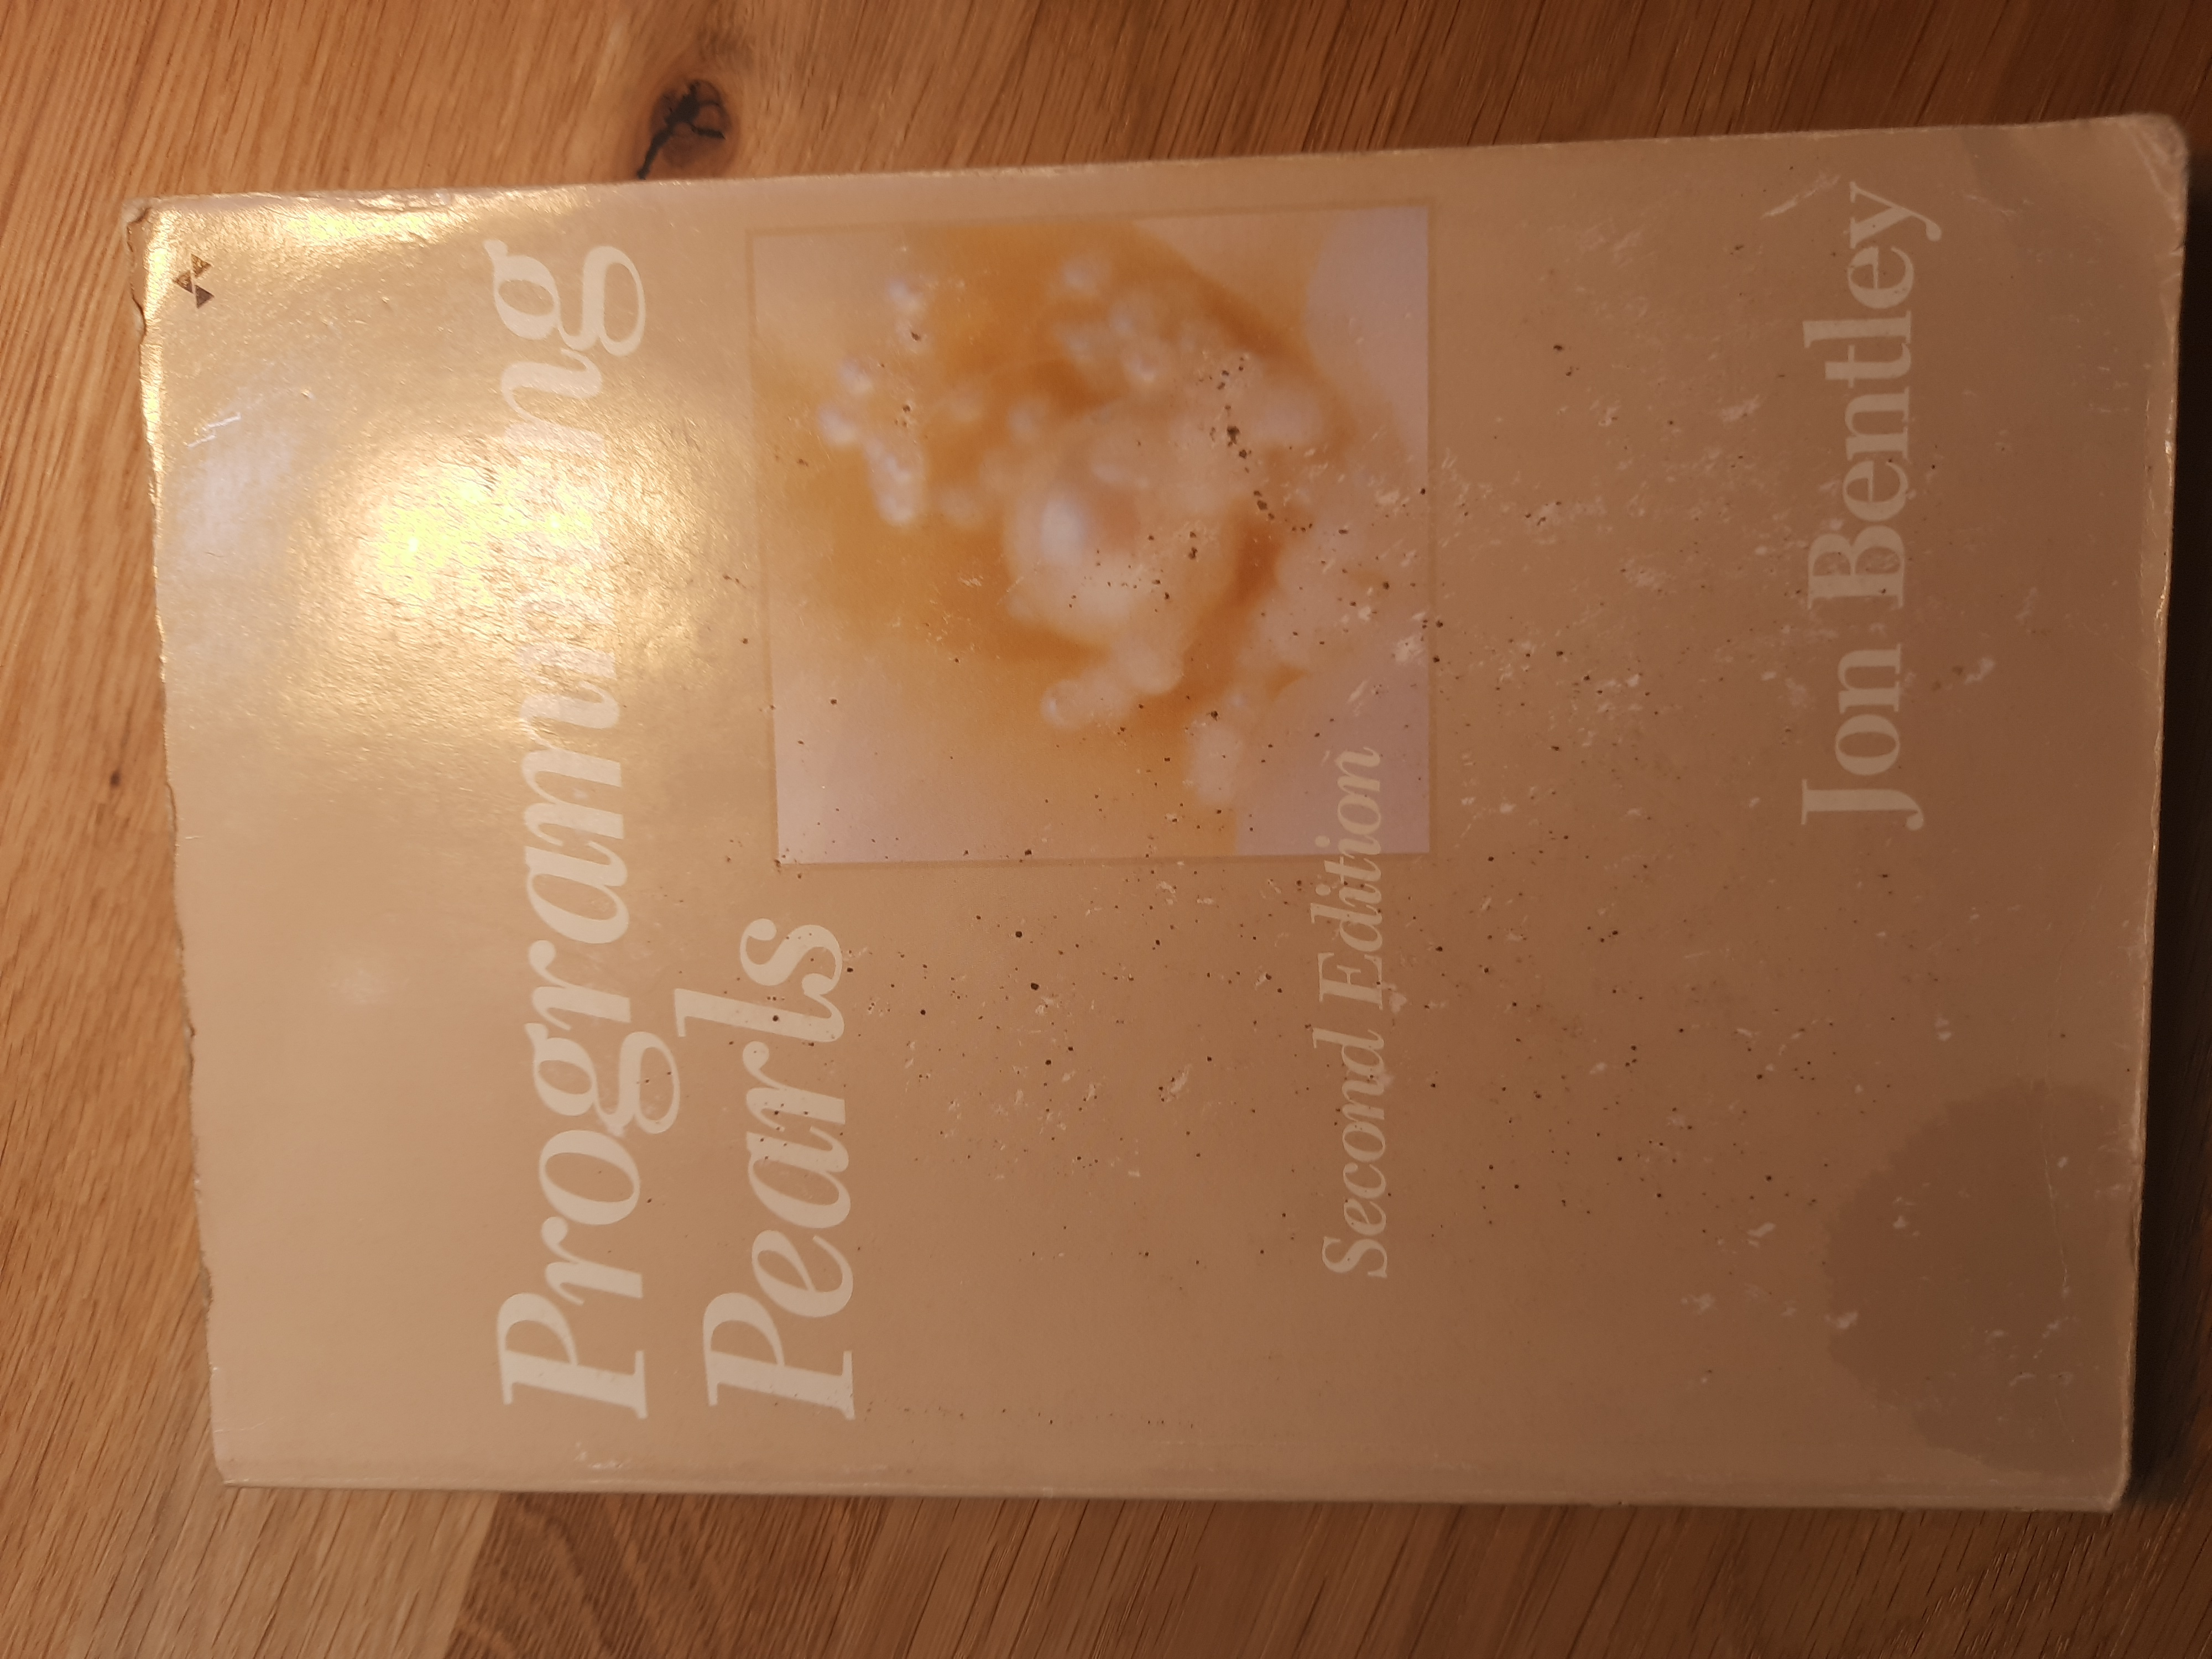
\includegraphics[width=\textwidth, height=\textheight, keepaspectratio=true]{programming_pearls}
\end{frame}

\begin{frame}
	\frametitle{Thinking a lot about Algorithms}
	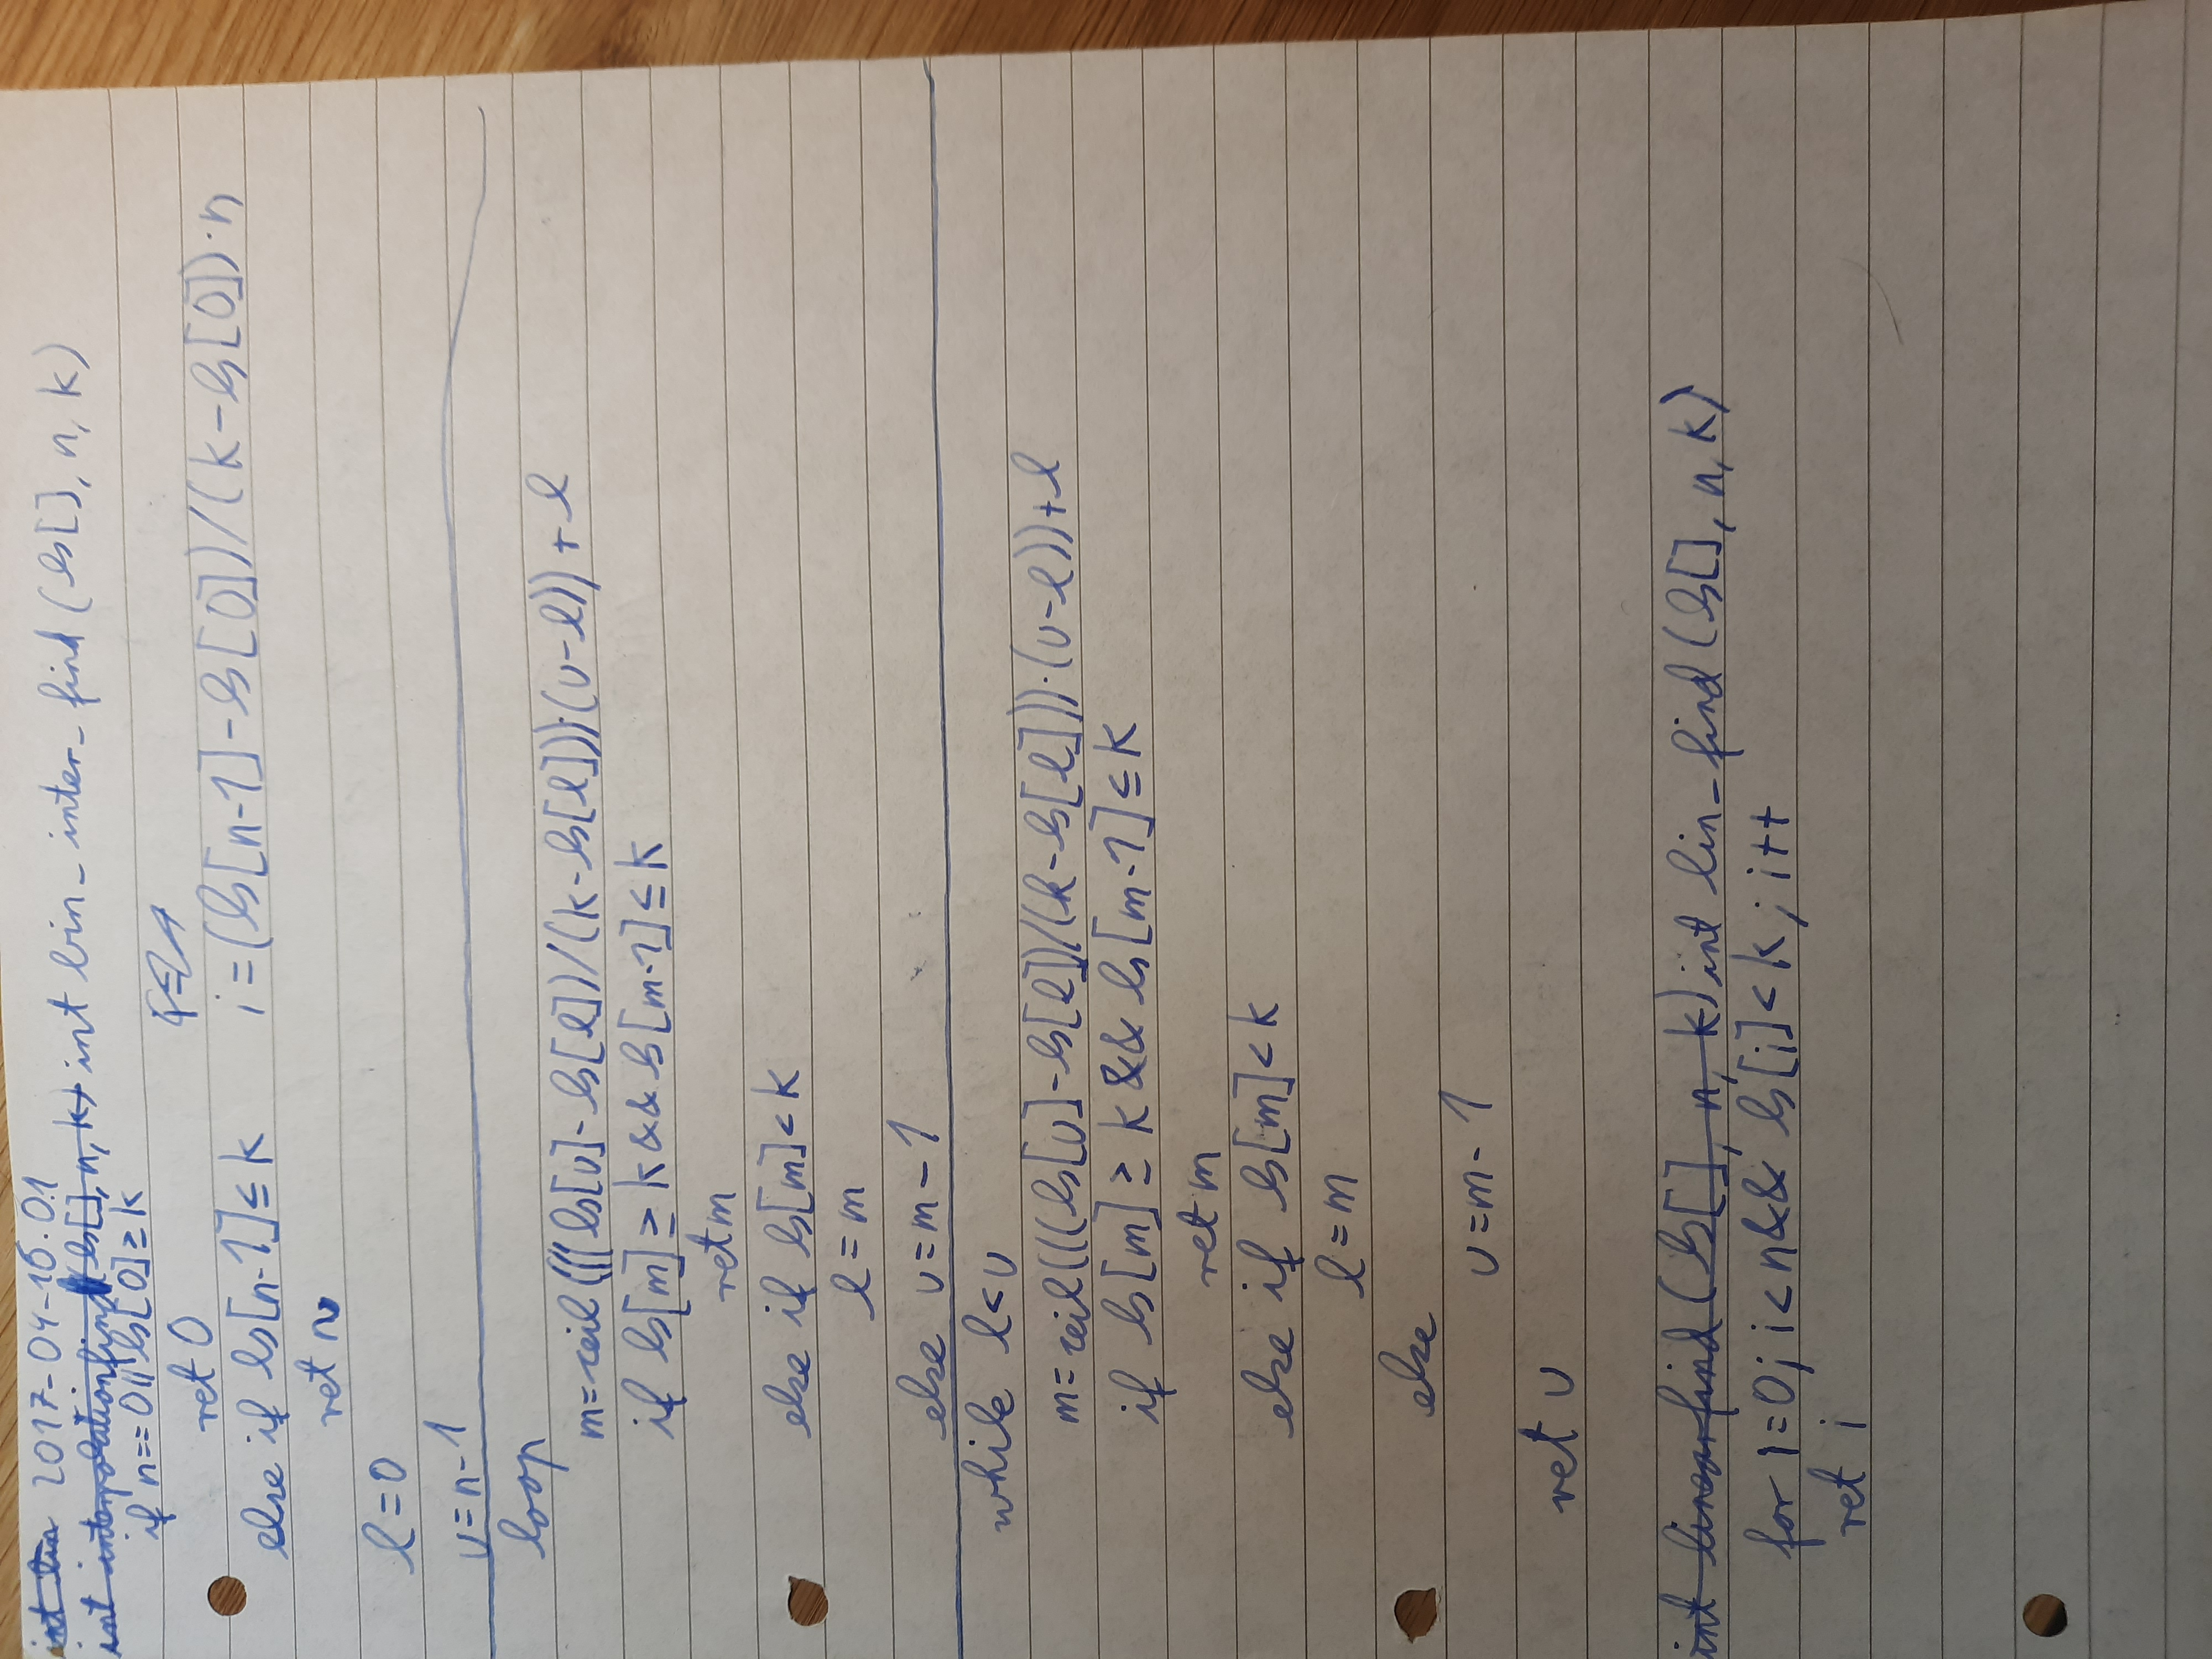
\includegraphics[width=\textwidth, height=\textheight, keepaspectratio=true]{nepal_search}
\end{frame}

\begin{frame}
	\frametitle{Problems back then}
	\begin{itemize}
		\item Thinking about searching, sorting, collision detection, string matching
		\item Specifically: What is the longest repeated substring of a string?
		\item Or: what is the longest supermaximal repeat of a string?
		\item Devising very complex algorithms
	\end{itemize}
\end{frame}

\begin{frame}
	\frametitle{Discovering Suffix Arrays}
	\begin{itemize}
		\item On the flight back reading the 15th chapter of Programming Pearls
		\item Describes this exact problem, solved using suffix arrays
	\end{itemize}
\end{frame}

\section{Structure}

\begin{frame}
	\frametitle{Structure of the Presentation}
	What, How, Why, in that order.
	\begin{itemize}
		\item Description of data structures
		\item Clarification of terminology
		\item Description of algorithms
		\item Discussion of advantages/disadvantages
	\end{itemize}
\end{frame}

\section{Data Structures}

\begin{frame}
	\frametitle{Contents of an Enhanced Suffix Array}
	\begin{itemize}
		\item Suffix Array $\hbox{suftab}$
		\item LCP Array $\hbox{lcptab}$
		\item Burrows-Wheeler Transformation Array $\hbox{bwttab}$
		\item Inverse Suffix Array $\hbox{suftab}^{-1}$
	\end{itemize}
\end{frame}

\begin{frame}
	\frametitle{Suffix Array $\hbox{suftab}$}
	Take string over finite alphatbet $\Sigma$, e.g. "cag" \\*
	Add character "\$" (is greater than any other character in $\Sigma$) \\*
	Sort suffixes \\*
	Positions of sorted suffixes in the string are entries of $\hbox{suftab}$
\end{frame}

\begin{frame}
	\frametitle{Example for $\hbox{suftab}$}
	For "cag" the suffixes are ("cag\$", \dq ag\$'', "g\$", "\$"). \\*
	The sorted suffixes: (\dq ag\$'', "cag\$", "g\$", "\$") \\*
	The suffix array then is $[1, 0, 2, 3]$
\end{frame}

\begin{frame}
	\frametitle{LCP Array $\hbox{lcptab}$}
	LCP Array is the array of the lengths for the prefixes of
	neighbouring suffixes in the suffix array

	More formal for a string $S$:

	$\hbox{lcptab}[i]=k \Leftrightarrow S[\hbox{suftab}[i]..\hbox{suftab}[i]+k]=S[\hbox{suftab}[i+1]..\hbox{suftab}[i+1]+k]$

	Value is $0$ for the last suffix.
\end{frame}

\begin{frame}
	\frametitle{LCP Array Example}
	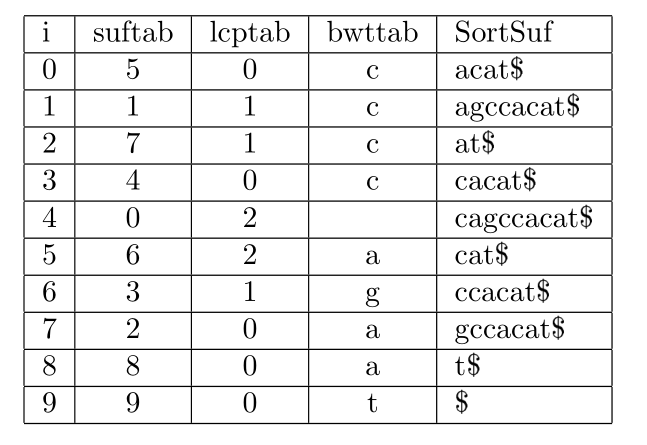
\includegraphics[width=\textwidth, height=\textheight, keepaspectratio=true]{esa_lcp_search}
\end{frame}

\begin{frame}
	\frametitle{Burrows-Wheeler Transformation Array $\hbox{bwttab}$}
	Informally, $\hbox{bwttab}$ contains the character before the
	suffix referenced in $\hbox{suftab}$.

	$\hbox{bwttab}[i]=c \Leftrightarrow S[suftab[i]-1]=c$

	Empty (or placeholder character) for the suffix that is also $S$.

	With BWT array, the Enhanced Suffix Array contains the whole
	string.
\end{frame}

\begin{frame}
	\frametitle{LCP Array with BWT Array Example}
        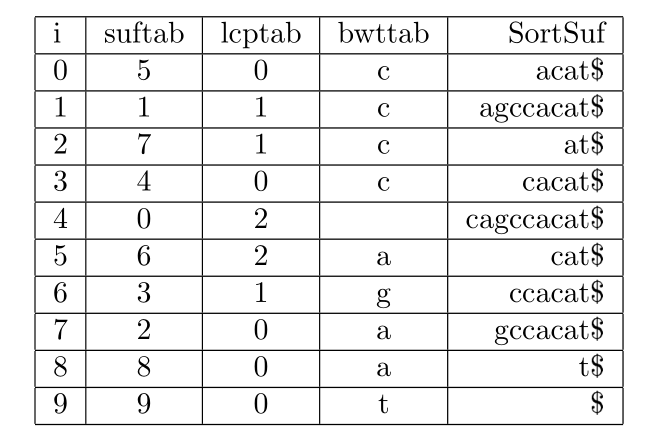
\includegraphics[width=\textwidth, height=\textheight, keepaspectratio=true]{esa_with_bwttab_example}
\end{frame}

\begin{frame}
	\frametitle{Inverse Suffix Array $\hbox{suftab}^{-1}$}
	Only sometimes part of the Enhanced Suffix Array.
	Is, as the name suggests, the inverse of the suffix array.

	$S[\hbox{suftab}^{-1}[\hbox{suftab}[i]]]=S[i]$.

	Example "cag":

	$\hbox{suftab}=[1,0,2,3]$, $\hbox{suftab}^{-1}=[0,1,3,2]$
\end{frame}

\begin{frame}
	\frametitle{LCP-Intervals}
	$\ell$-interval: Roughly an interval in the LCP array where the LCP value is always
	$\ge \ell$, and which is surrounded by LCP values $< \ell$.\\*

	\vspace{5mm}
	More formally:
	The interval $[i..j]$ is an LCP-interval of value $\ell$ (short $\ell-[i..j]$)
	iff \\*
	\begin{itemize}
		\item $\hbox{lcptab}[i]<\ell$
		\item $\hbox{lcptab}[k]\ge \ell$ for all $k: i+1 \le k \le j$
		\item $\hbox{lcptab}[k=\ell$ for at least one $k: i+1 \le k \le j$
		\item $\hbox{lcptab}[j+1]<\ell$
	\end{itemize}
\end{frame}

\begin{frame}
	\frametitle{Example for an $\ell$-Interval}
	$1-[4..6]$ is an LCP interval, $2-[4..5]$ is also an interval
	(note that they are embedded in each other!
	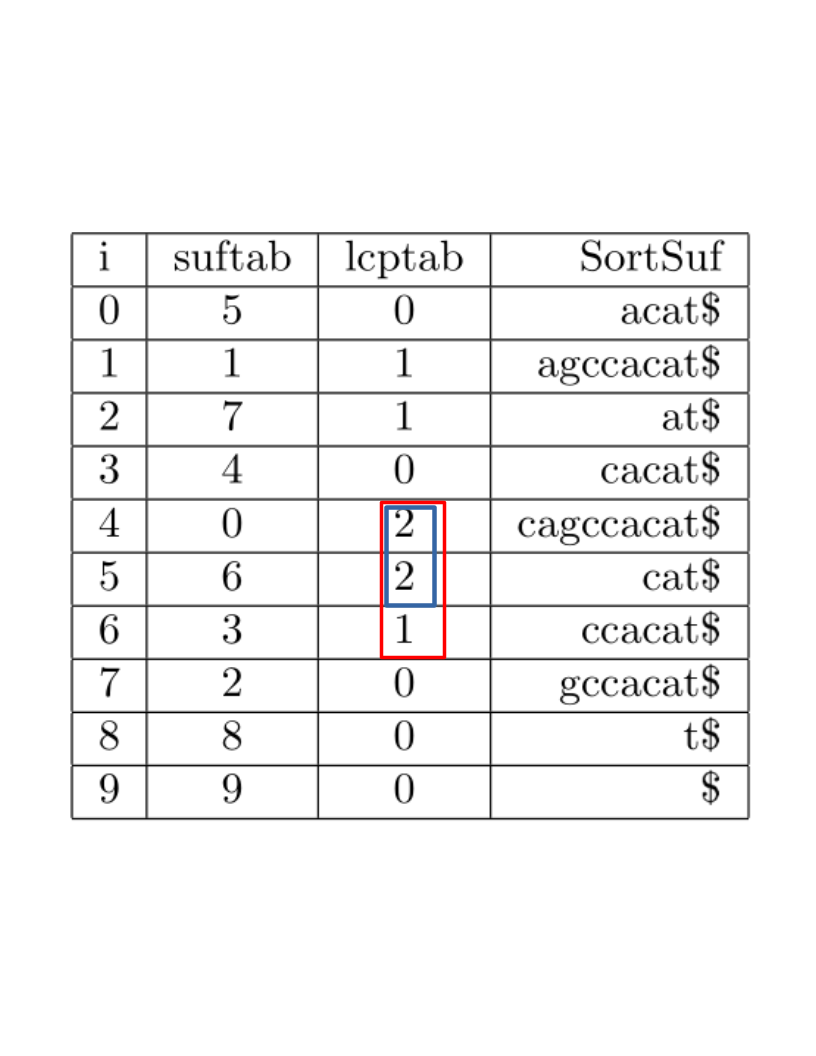
\includegraphics[width=\textwidth, height=\textheight, keepaspectratio=true]{esa_example_highlight_interval}
\end{frame}

\begin{frame}
	\frametitle{LCP-Interval Trees}
	LCP-intervals are embedded within each other, a $1$-interval
	can contain a $2$-interval.

	This forms a so-called LCP-interval tree: the root contains the $0$-interval,
	then the $1$-intervals in the next level, \& so on.
\end{frame}

\begin{frame}
	\frametitle{LCP-Interval Tree for given string}
	\includegraphics[width=\textwidth, height=\textheight, keepaspectratio=true]{LCP_interval_tree}
\end{frame}

\begin{frame}
	\frametitle{LCP-Intervals not part of the Enhanced Suffix Array}
	\cite{abouelhoda2002enhanced} stresses repeatedly that neither
	LCP-intervals nor LCP-interval trees are stored, they are merely
	inferred by LCP array \& BWT array.
\end{frame}

\section{Terminology}

\begin{frame}
	\frametitle{Enhanced Suffix Array vs. Extended Suffix Array}
	Terminology a bit jumbled…

	We have:
	\begin{itemize}
		\item Suffix Array: Introduced by \cite{manber1993suffix} (but likely used before), only contains suffix array
		\item Suffix Array with LCP-Array: Very common, also mentioned by \cite{manber1993suffix} and \cite{gusfield1997algorithms}
		\item Extended Suffix Array: Rarely used, only mentioned by \cite{salson2010dynamic}, seems to be just suffix array with LCP array.
		\item Enhanced Suffix Array: Introduced by \cite{abouelhoda2002enhanced}, \textbf{focus of this talk}. Contains suffix array, BWT array, LCP array
	\end{itemize}
\end{frame}

\begin{frame}
	\frametitle{In Short}
	\begin{itemize}
		\item There's Suffix Arrays
		\item There's Suffix Arrays with LCP Information=Extended Suffix Arrays
		\item There's Enhanced Suffix Arrays (Suffix Arrays with LCP \& more)
	\end{itemize}
\end{frame}

\section{Algorithms}

\begin{frame}
	\frametitle{Many Different String Matching Problems}
	\begin{itemize}
		\item Exact String Matching
		\item Finding Maximal/Supermaximal Repeats
		\item Finding Longest Common Substring (of $\ge 2$ strings)
	\end{itemize}
	Many of these can be implemented by traversal of LCP-interval tree.
\end{frame}

\begin{frame}
	\frametitle{Exact String Matching (Substring Search)}
	Find all occurrences of $T$ in $S$.

	Or, more formal: Given strings $S$ and $T$ of lengths $n$ and
	$m$, $m \le n$, return indices $I=\{i_{1}, \ldots, i_{k}\}$
	so that $\forall i \in I: S[i..i+m]=T$
\end{frame}

\begin{frame}
	\frametitle{Using only the Suffix Array}
	There exists an interval in the suffix array (possibly empty)
	where $T$ is the prefix of the referenced suffixes.

	Use binary search to find the starting position of that interval,
	then another binary search to find the end position.

	Second search uses start position of the interval as left
	starting point.

	Runtime $\O(m + \log n)$ (\cite{manber1993suffix}).
\end{frame}

\begin{frame}
	\frametitle{Example}
	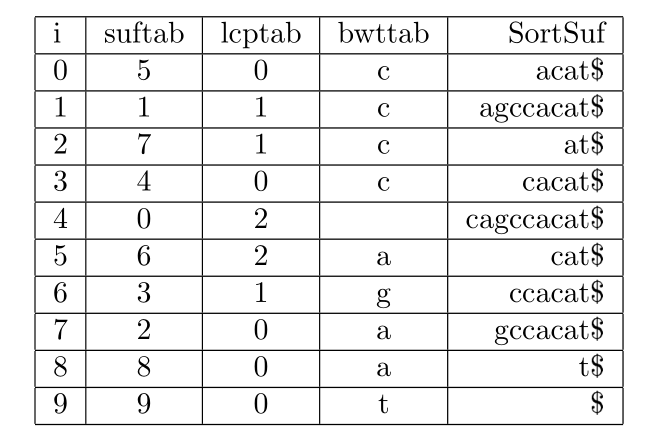
\includegraphics[width=\textwidth, height=\textheight, keepaspectratio=true]{esa_with_bwttab_example}
\end{frame}

\begin{frame}
	\frametitle{Using the Suffix Array with LCP information}
	\cite{manber1993suffix} already describes methods of speeding
	this binary search up using LCP information:

	When the upper and lower bound lie within
	the same $\ell$-interval, comparing $T$ and
	$S[\hbox{suftab}[\hbox{mid}]]$ is can be started at position
	$T[\ell]$, $S[\hbox{suftab}[\hbox{mid}]+\ell]$.
\end{frame}

\begin{frame}
	\frametitle{Generating the LCP Information}
	For this, \cite{manber1993suffix} proposes pre-computing LCP
	information for binary-tree-like pairs
	($(0,n), (0,\frac{n}{2}), (\frac{n}{4}, \frac{3*n}{4})$ etc.),
	but there are other possible approaches, using e.g. traversal
	of LCP-interval trees.
\end{frame}

\begin{frame}
	\frametitle{Example}
	$T$="cac", $\hbox{low}=3$, $\hbox{high}=6$.
	\includegraphics[width=\textwidth, height=\textheight, keepaspectratio=true]{esa_LCP_search_1}
\end{frame}

\begin{frame}
	\frametitle{Gusfield's Super-Accelerant}
	\cite[pp. 152]{gusfield1997algorithms} describes a further
	accelerant to searching using LCP data.
	%TODO: understand it & describe it here!

	Note that these accelerants don't improve worst-case performance,
	which is still $\O(m + \log n)$.
\end{frame}

\begin{frame}
	\frametitle{Personal Idea}
	Personal idea: use Interpolation Search
	(\cite{perl1978interpolation}) for searching the suffix array.

	Reasons: runs in $\O(\log \log n)$ average case, and genomic
	data seems uniformly distributed.
\end{frame}

\begin{frame}
	\frametitle{Finding Supermaximal Repeats}
	Finding supermaximal repeats is comparatively easy

	\dq A string $\omega$ is a supermaximal repeat if[f] […] there is an
        $\ell$-interval [i..j] such that
	\begin{itemize}
		\item[–] [i..j] is a local maximum in the LCP-table and [i..j] is the $\omega$-interval,
		\item[–] the characters bwttab[i], bwttab[i+1], …, bwttab[j] are pairwise distinct."
	\end{itemize}
	\cite{abouelhoda2002enhanced}
\end{frame}

\begin{frame}
	\frametitle{Algorithm}
	Traverse LCP-array linearly, whenever finding a local maximum
	(and $\hbox{bwttab}[i] \neq \hbox{bwttab}[i+1]$), report it.

	Runs in $\O(n)$.
\end{frame}

\begin{frame}
	\frametitle{Illustration}
	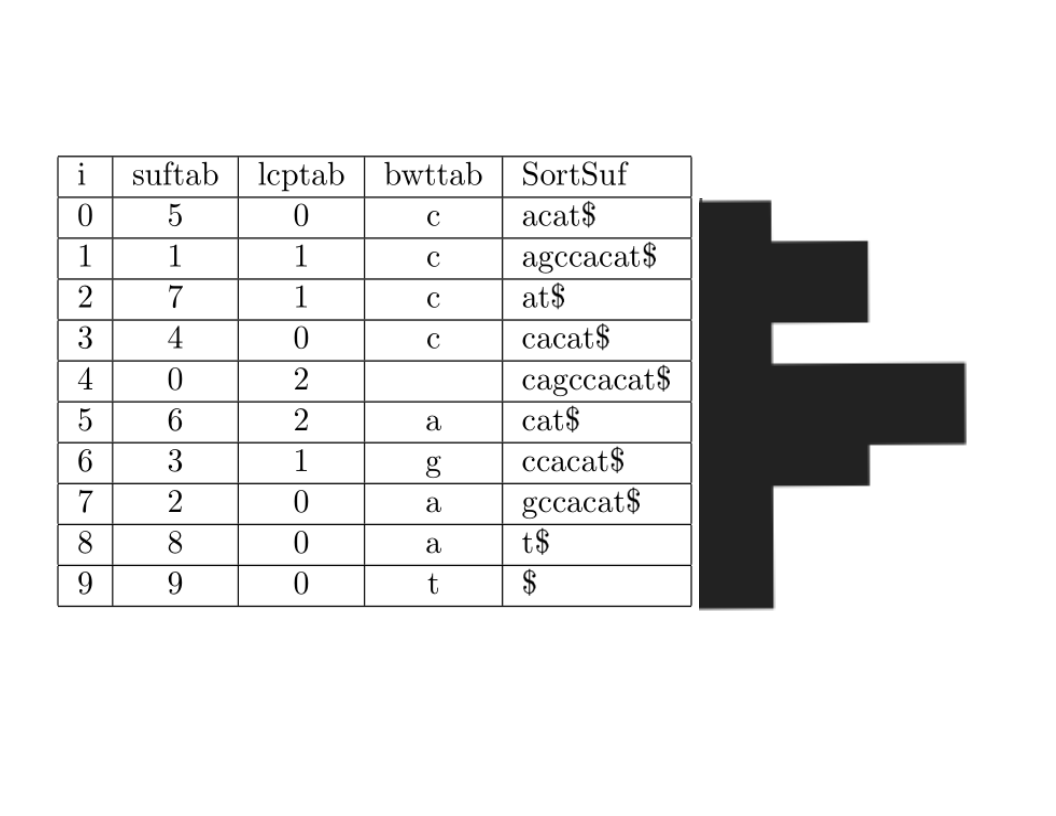
\includegraphics[width=\textwidth, height=\textheight, keepaspectratio=true]{local_maxima}
\end{frame}

\begin{frame}
	\frametitle{Finding Maximum Unique Matches}
	In short, a Maximum Unique Match (MUM) is just a supermaximal
	repeat in two different strings.

	Or, more formally: The MUM $u$ of $S_1$ and $S_2$
	is a supermaximal repeat of $S_1\#S_2$ so that
	$(i_1,j_1)=(i_2,j_2)=u$ and $j_1<p<i_2$ ($p=|S_1|$).
\end{frame}

\begin{frame}
	\frametitle{Algorithm for finding MUMs}
	Use the algorithm for finding supermaximal repeats on $S_1\#S_2$.

	Filter out non-MUM matches.

	Runs in $\O(n)$.

	But: This seems very wasteful to me! Every time we want to
	calculate a MUM, we have to generate the ESA for the whole
	$S_1\#S_2$! Especially if computing MUMs for many different
	$S_2$, this seems horrible! But maybe clever trick for combining
	ESAs? Haven't seen it yet.
\end{frame}

\subsection{Traversing the lcp-interval tree}

\begin{frame}
	\frametitle{traversing the lcp-interval tree}
	The lcp-interval tree is very useful many kinds of strings
	processing algorithms.

	It is the suffix tree without leaves.

	Is {\em{never actually completely constructed}}, but {\em{instead
	generated on the fly from the lcp array}}.
\end{frame}

\begin{frame}
	\frametitle{Algorithm for traversing the lcp-interval tree}
	In essence:

	\begin{itemize}
		\item the "level" we're on in the lcp-interval describes the current position in the tree
		\item we can save child intervals on a stack
		\item Whenever we "leave\dq an interval, we
		\item \begin{itemize}
			\item Pop it from the stack
			\item Process it <-- Customizable!
			\item Add it to the list of child intervals of the top element of the stack
		\end{itemize}
		\item Whenever we \dq enter\dq a new interval, we push it on the stack
	\end{itemize}
\end{frame}

\begin{frame}
	\frametitle{Example}
	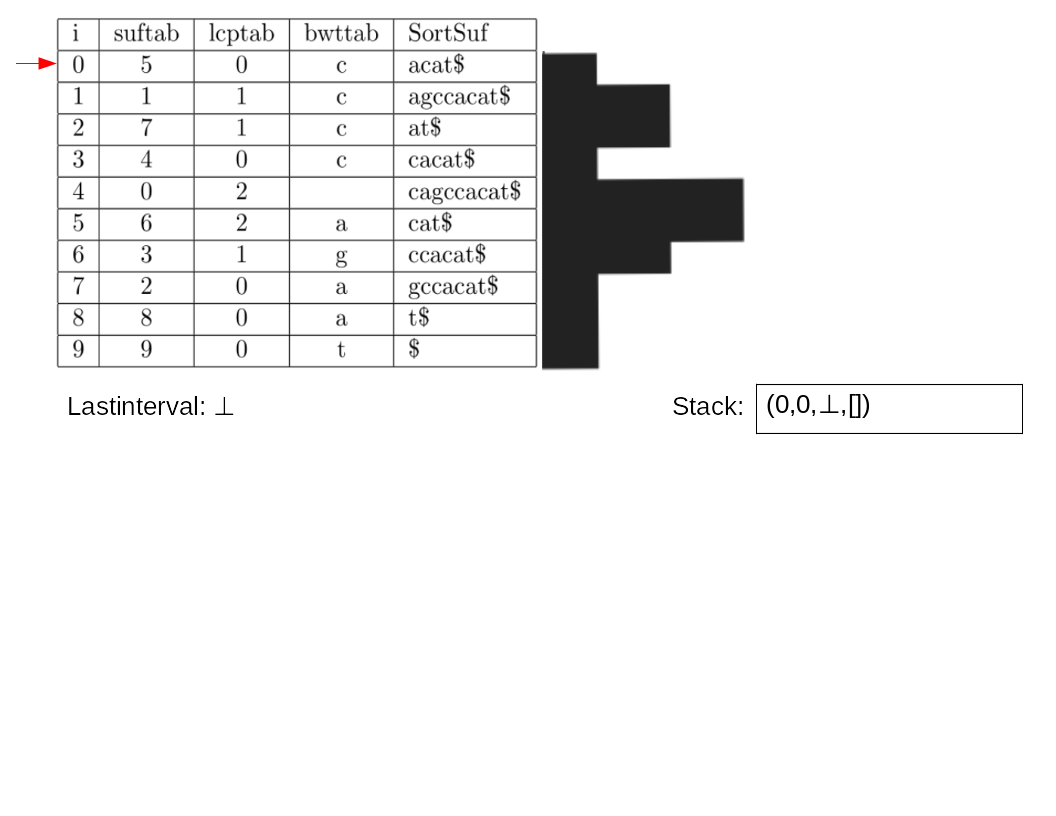
\includegraphics[width=\textwidth, height=\textheight, keepaspectratio=true]{traversal_1}
\end{frame}

\begin{frame}
	\frametitle{Example}
	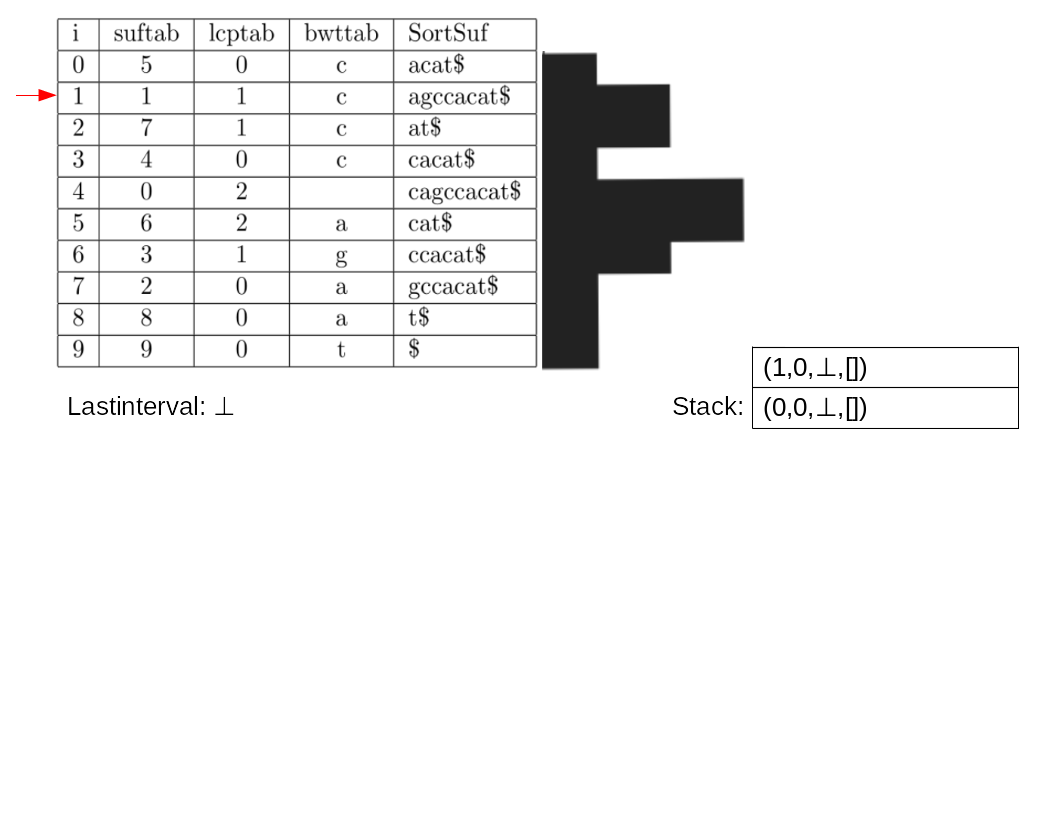
\includegraphics[width=\textwidth, height=\textheight, keepaspectratio=true]{traversal_2}
\end{frame}

\begin{frame}
	\frametitle{Example}
	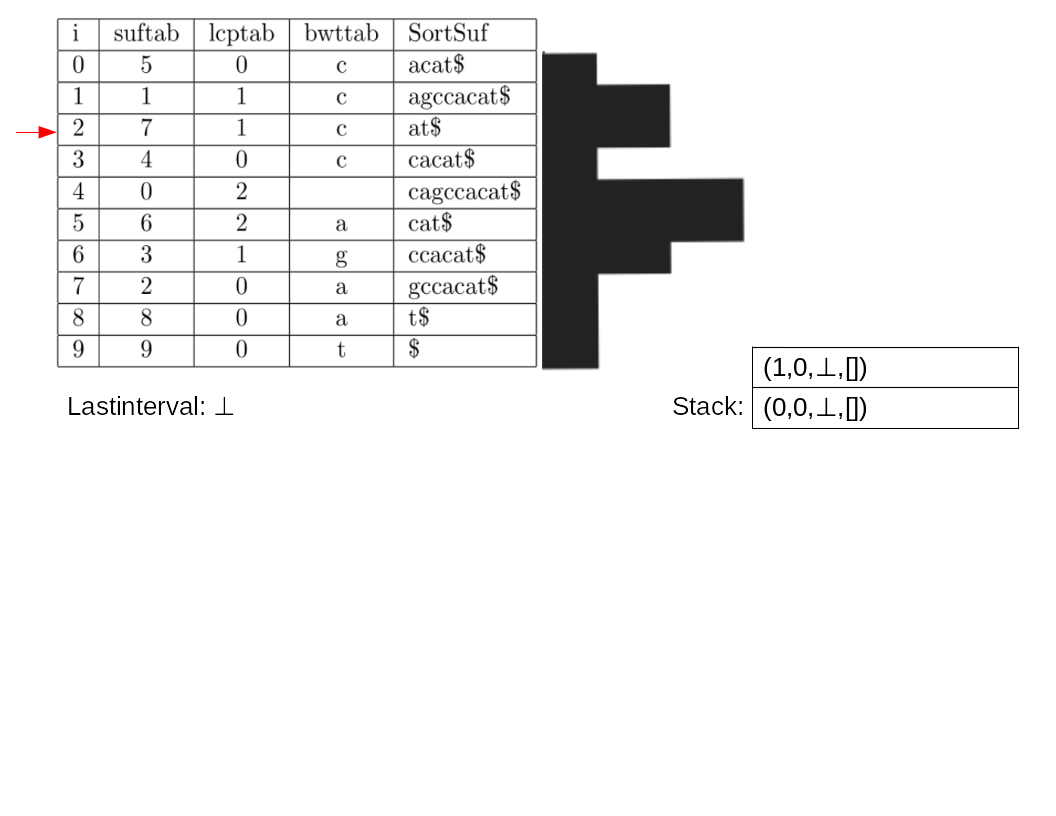
\includegraphics[width=\textwidth, height=\textheight, keepaspectratio=true]{traversal_3}
\end{frame}

\begin{frame}
	\frametitle{Example}
	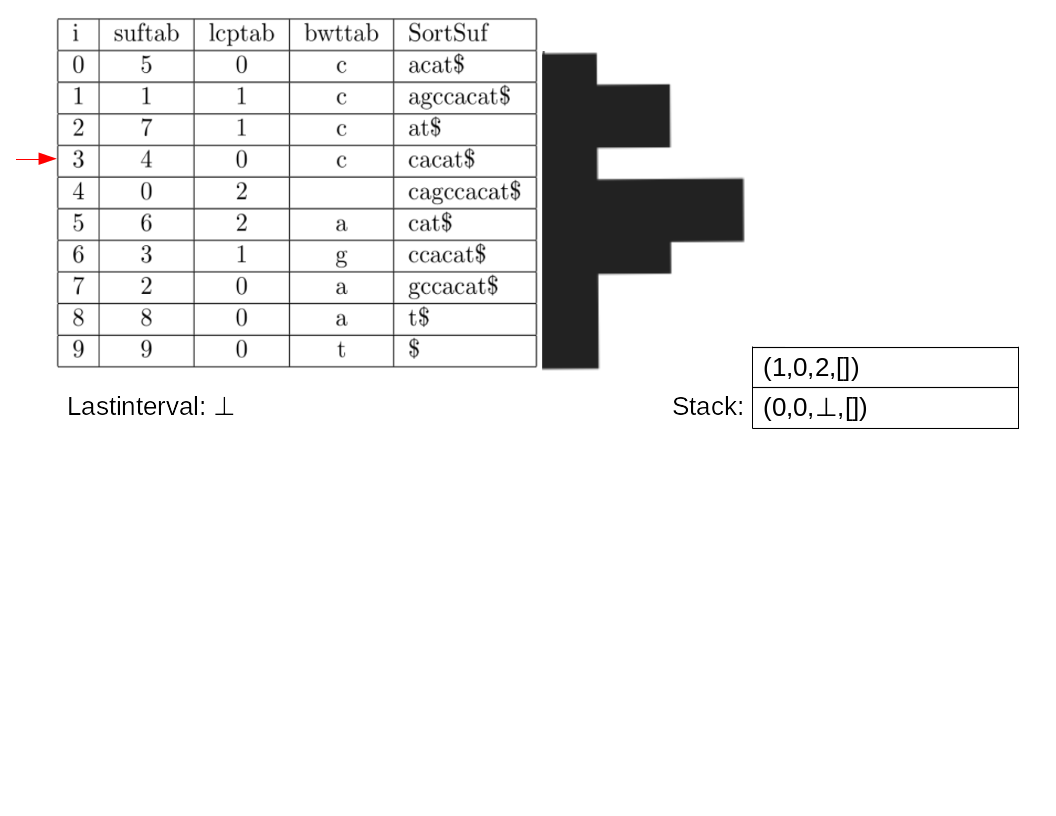
\includegraphics[width=\textwidth, height=\textheight, keepaspectratio=true]{traversal_4}
\end{frame}

\begin{frame}
	\frametitle{Example}
	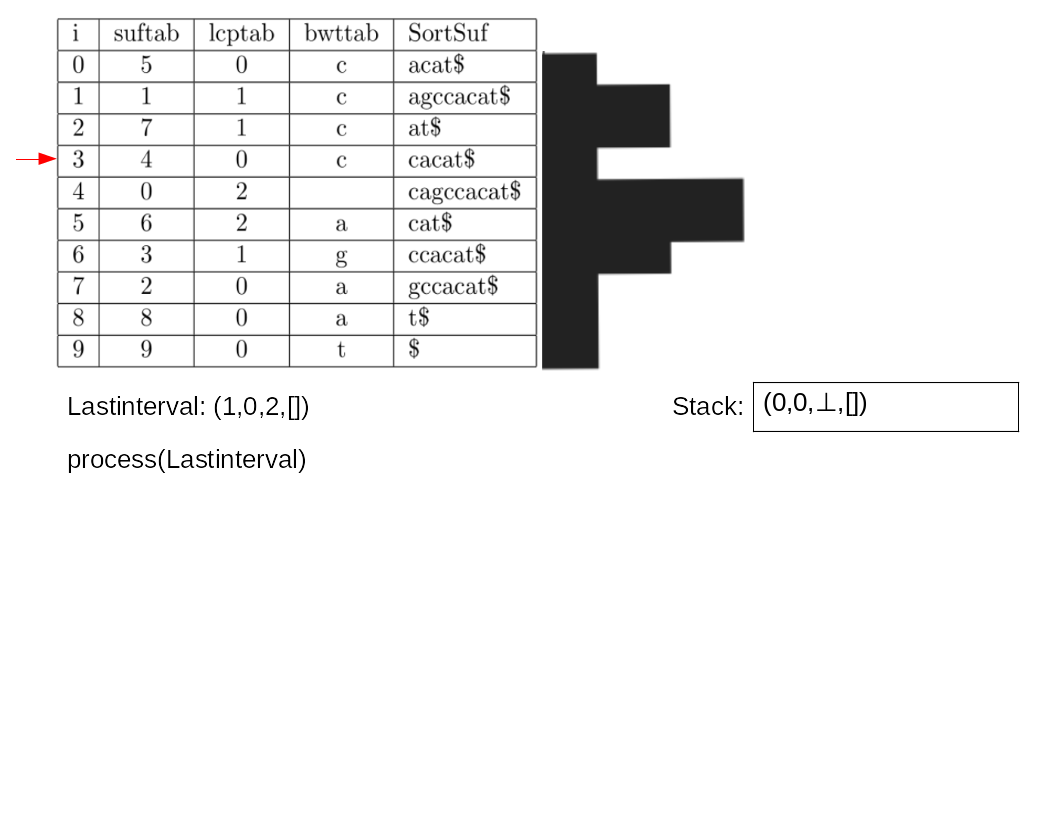
\includegraphics[width=\textwidth, height=\textheight, keepaspectratio=true]{traversal_5}
\end{frame}

\begin{frame}
	\frametitle{Example}
	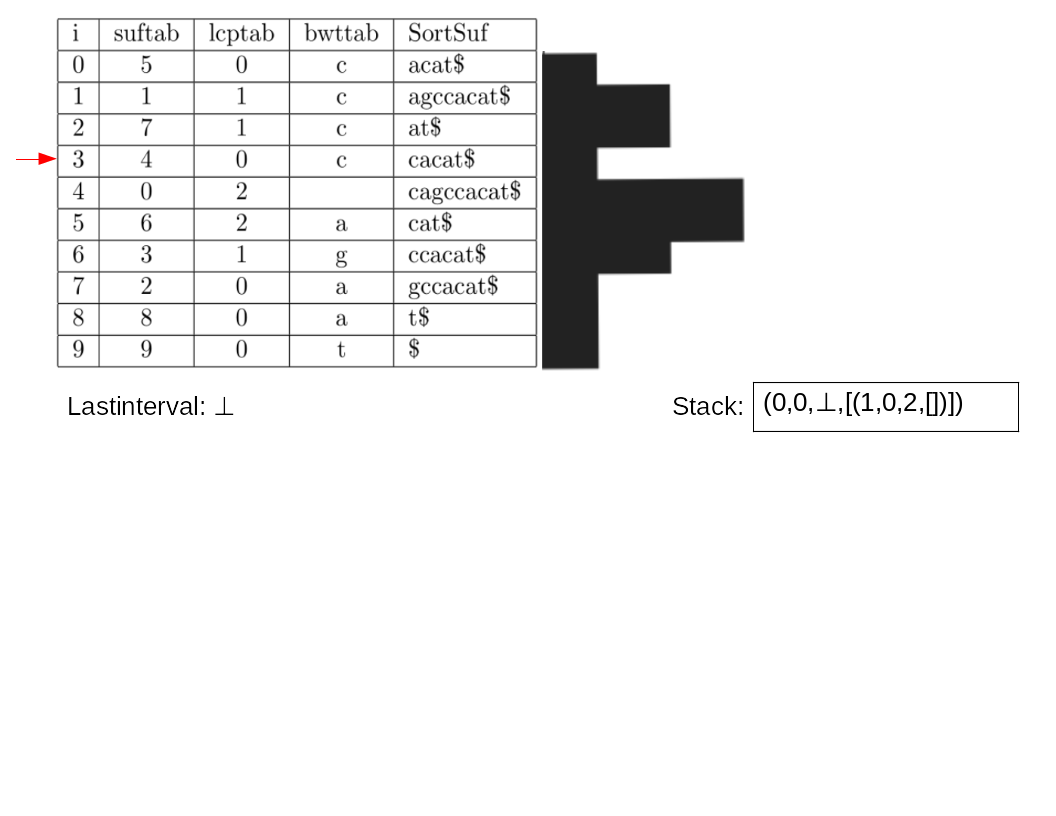
\includegraphics[width=\textwidth, height=\textheight, keepaspectratio=true]{traversal_6}
\end{frame}

\begin{frame}
	\frametitle{Example}
	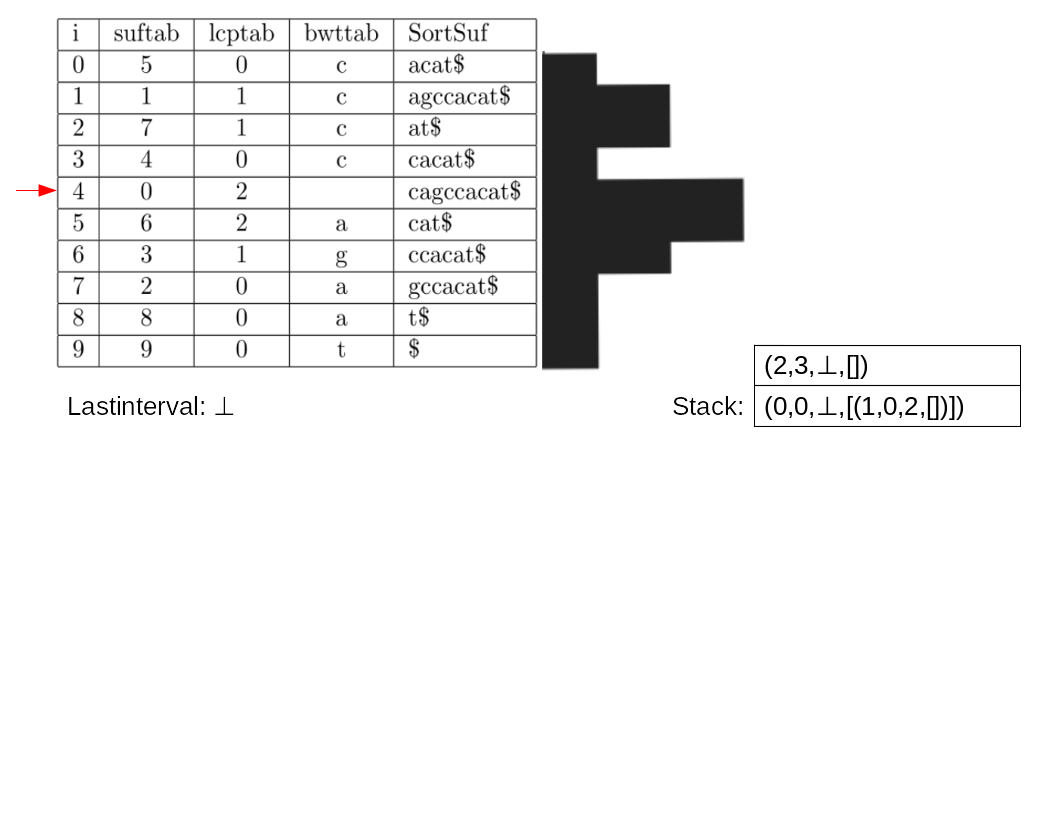
\includegraphics[width=\textwidth, height=\textheight, keepaspectratio=true]{traversal_7}
\end{frame}

\begin{frame}
	\frametitle{Example}
	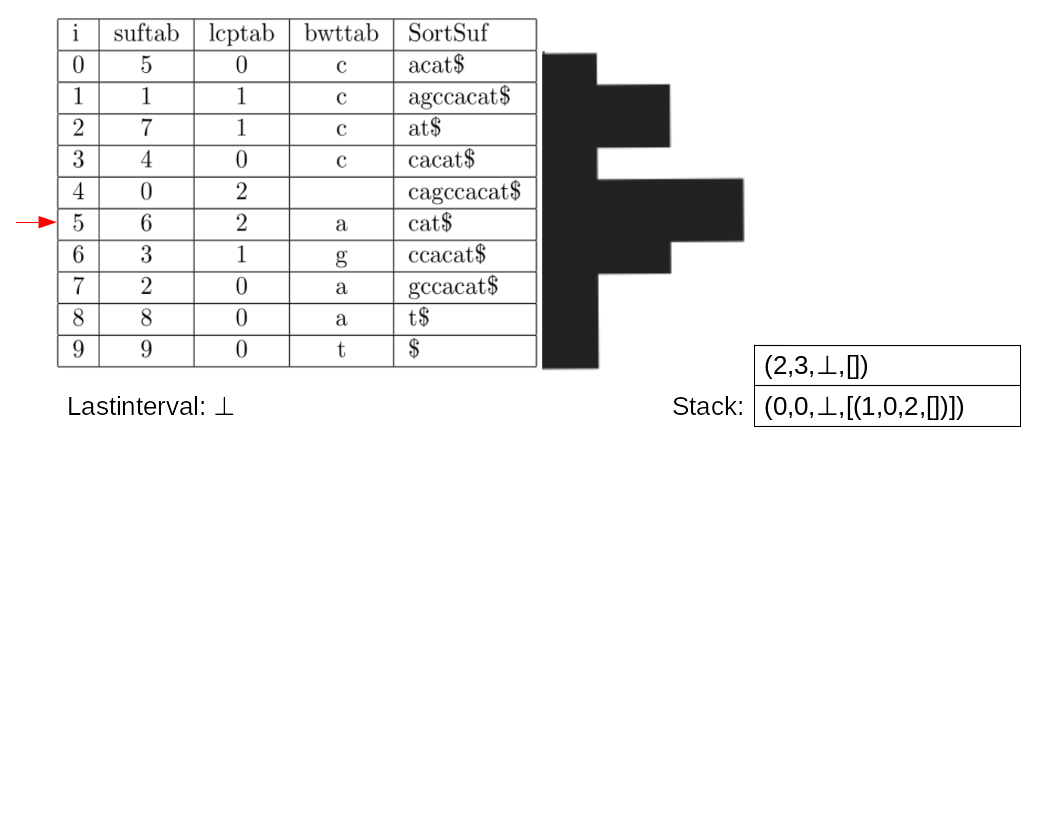
\includegraphics[width=\textwidth, height=\textheight, keepaspectratio=true]{traversal_8}
\end{frame}

\begin{frame}
	\frametitle{Example}
	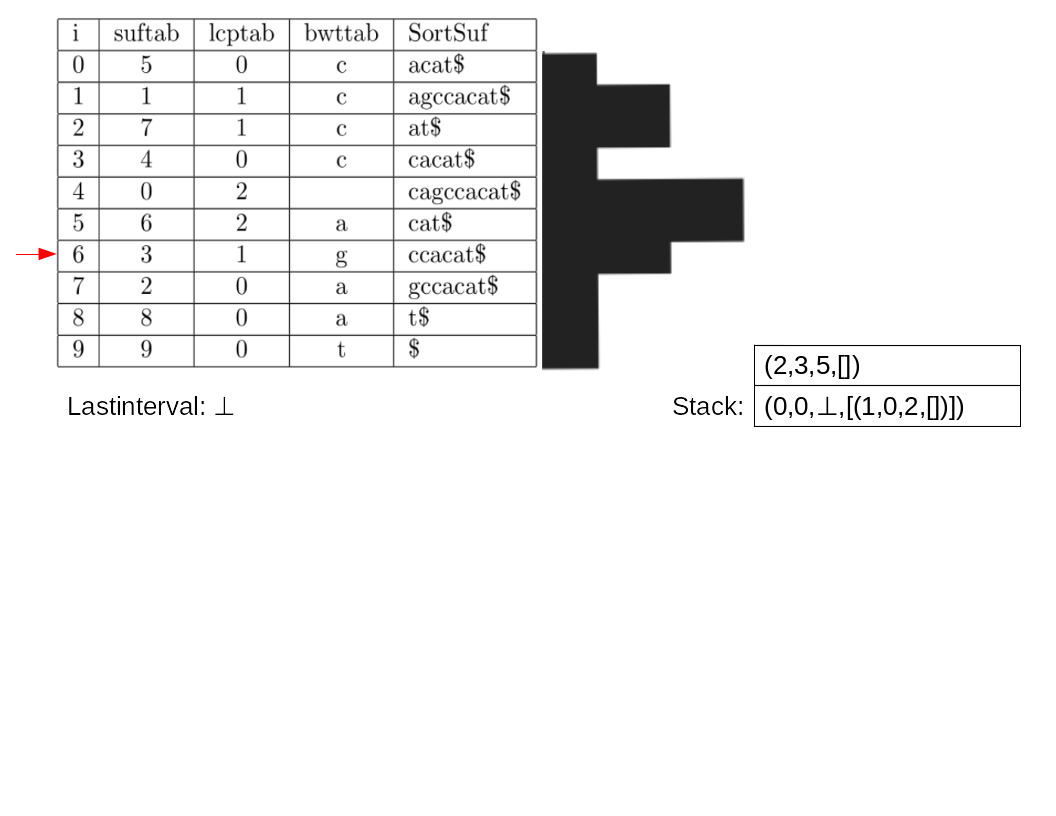
\includegraphics[width=\textwidth, height=\textheight, keepaspectratio=true]{traversal_9}
\end{frame}

\begin{frame}
	\frametitle{Example}
	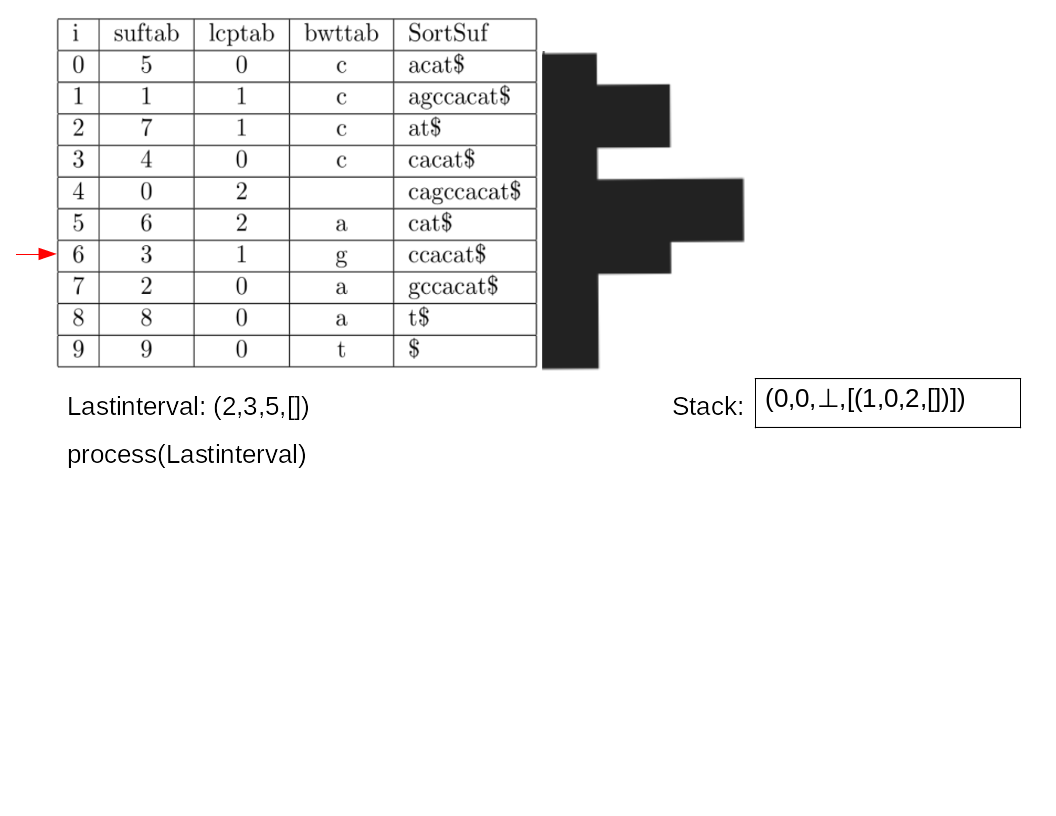
\includegraphics[width=\textwidth, height=\textheight, keepaspectratio=true]{traversal_10}
\end{frame}

\begin{frame}
	\frametitle{Example}
	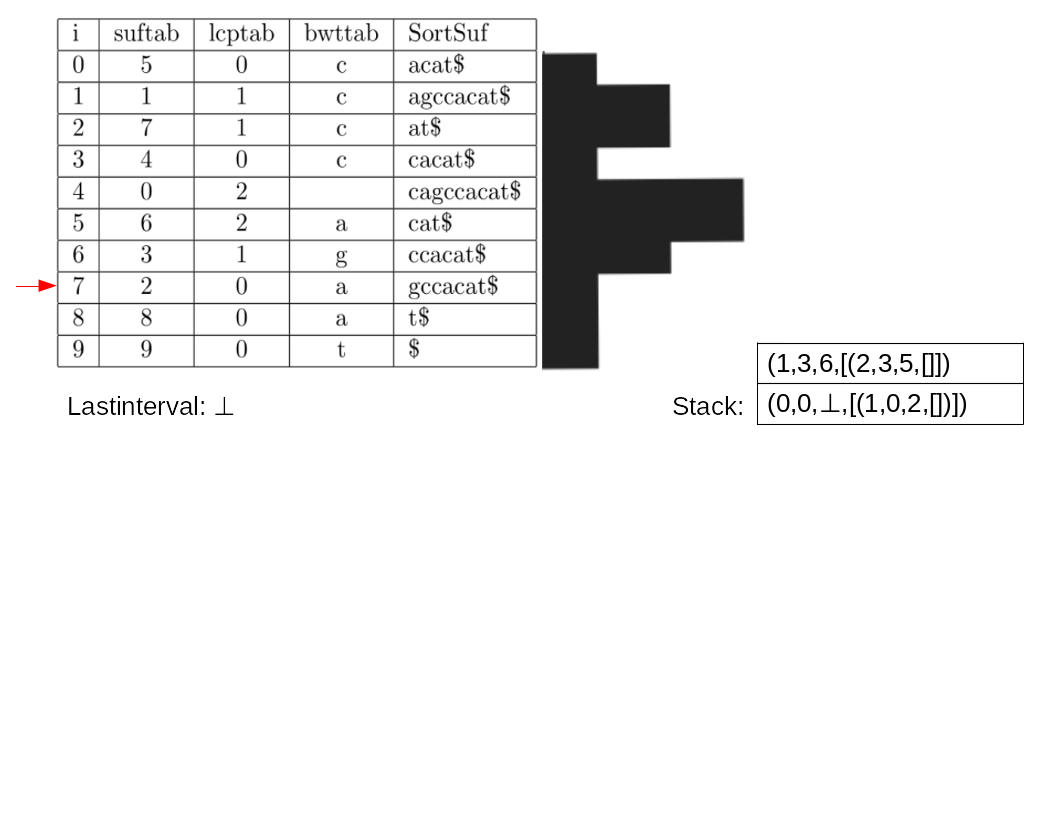
\includegraphics[width=\textwidth, height=\textheight, keepaspectratio=true]{traversal_11}
\end{frame}

\begin{frame}
	\frametitle{Example}
	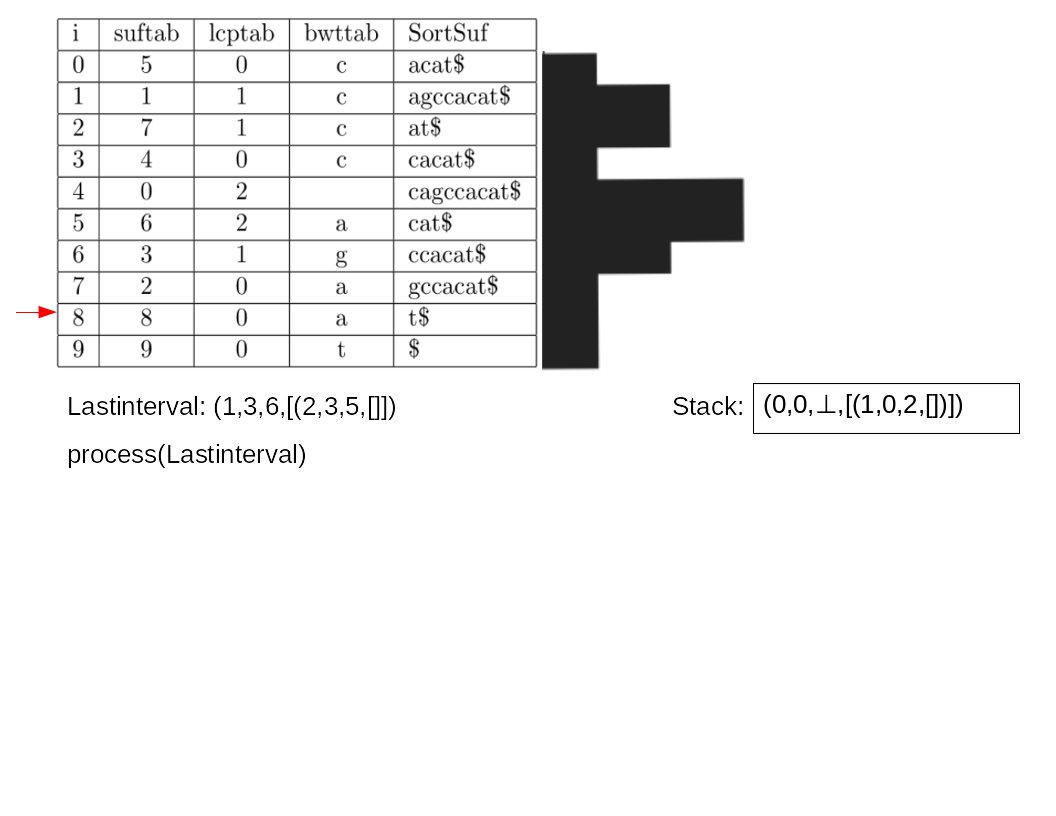
\includegraphics[width=\textwidth, height=\textheight, keepaspectratio=true]{traversal_12}
\end{frame}

\begin{frame}
	\frametitle{Example}
	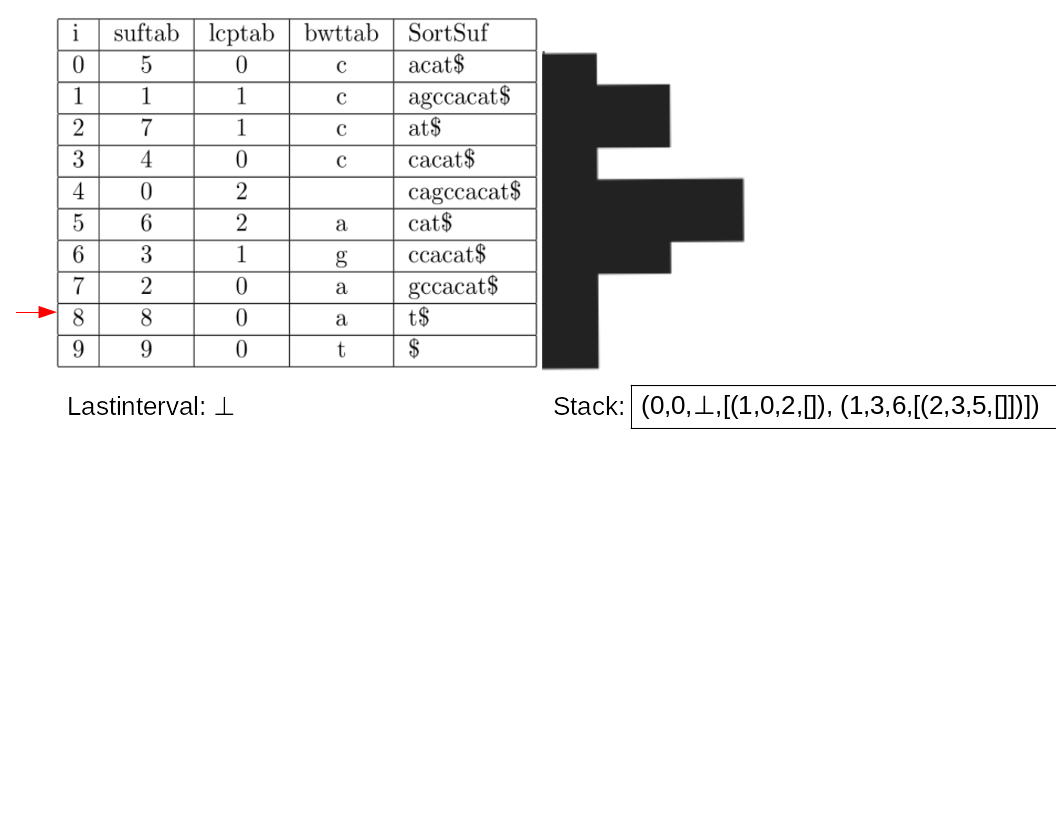
\includegraphics[width=\textwidth, height=\textheight, keepaspectratio=true]{traversal_13}
\end{frame}

\begin{frame}
	\frametitle{Example}
	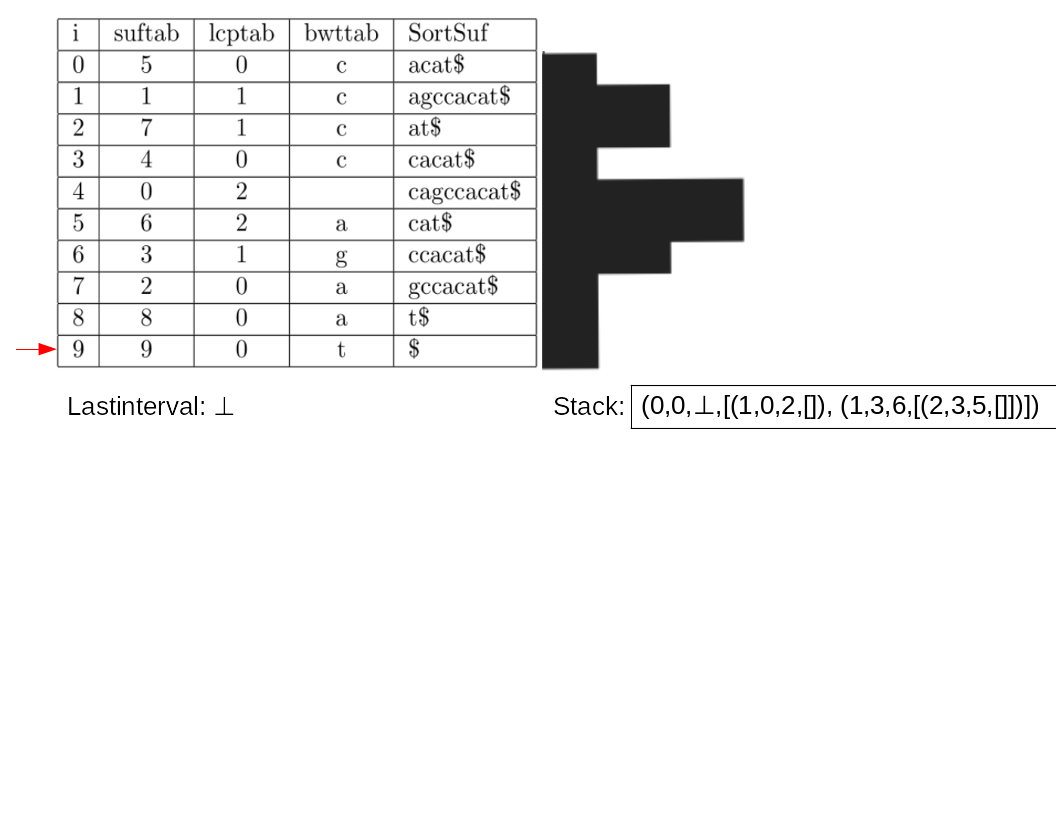
\includegraphics[width=\textwidth, height=\textheight, keepaspectratio=true]{traversal_14}
\end{frame}

\begin{frame}
	\frametitle{Example}
	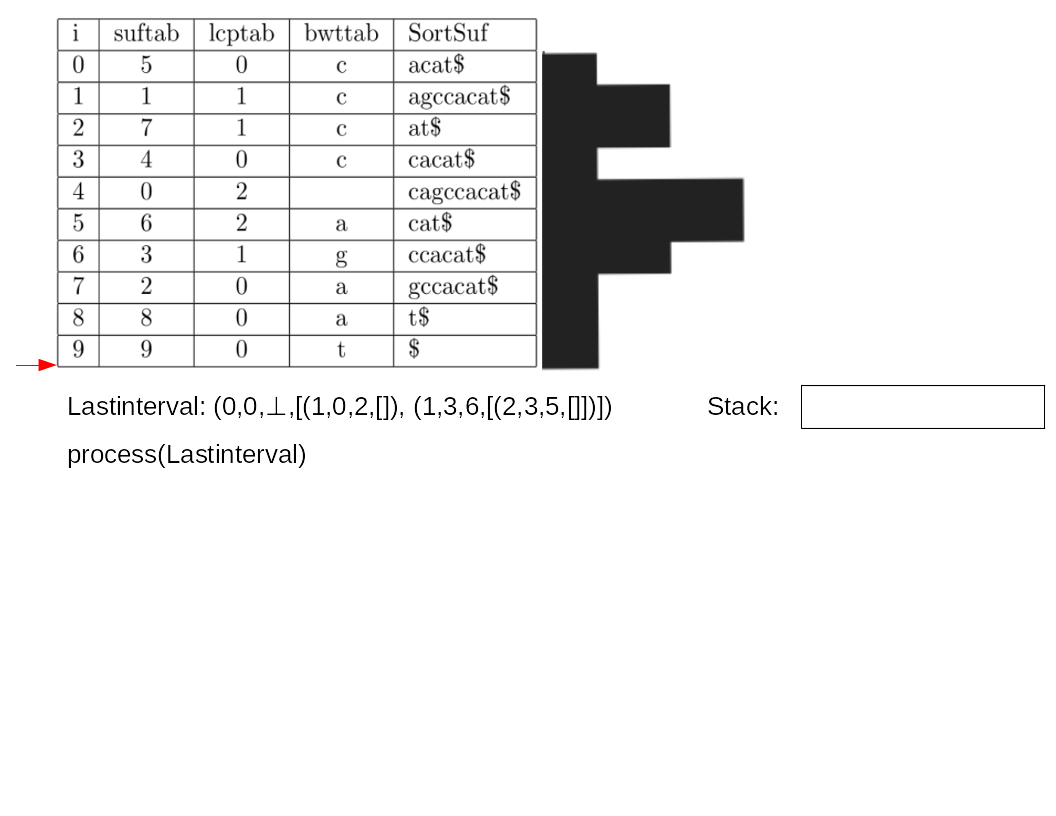
\includegraphics[width=\textwidth, height=\textheight, keepaspectratio=true]{traversal_15}
\end{frame}

\begin{frame}
	\frametitle{Processing an Interval}
	The magic happens in the function process, which could be given
	as a parameter to the algorithm.

	It receives an lcp-interval, containing:
	\begin{itemize}
		\item $\ell$-value (length of prefixes)
		\item Left and right boundary of the interval
		\item List of children of the interval
	\end{itemize}
\end{frame}

\begin{frame}
	\frametitle{Properties of LCP-Interval Tree Traversal}
	Runtime depends on
	\begin{itemize}
		\item Time for specific data structures (list for children, stack)
		\item Time complexity for process
	\end{itemize}

	In itself, it has a runtime of $\O(n)$.
\end{frame}

\begin{frame}
	\frametitle{Maximal Repeats}
	A maximal repeat is a string $\omega$ so that
	$\omega=S[i_1..j_1]=S[i_2..j_2]$, with $i_1 \ne i_2$, and both
	$S[i_1-1] \ne S[i_2-1]$ and $S[j_1+1] \ne S[j_2+1]$.

	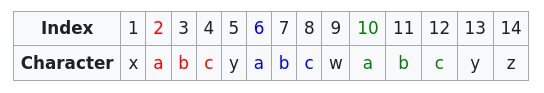
\includegraphics[width=\textwidth, height=\textheight, keepaspectratio=true]{maximal_pair}

%TODO: space!
	Here, \dq abc\dq is a maximal repeat, but \dq abcy\dq is a supermaximal
	repeat.
\end{frame}

\begin{frame}
	\frametitle{Computing Maximal Repeats}
	This algorithm uses the lcp-interval tree traversal, so we start
	in the function process that receives an lcp-interval.

	Runs in $\O(kn+z)$, $k=|\Sigma|$, $z$ number of maximal repeated
	pairs, $n=|S|$.
\end{frame}

\begin{frame}
	\frametitle{Position Sets}
	Broadly, for every $\ell$-interval the algorithm attempts to
	find the set of all positions in the interval preceded by the
	character $a$, $\forall a \in \Sigma$.

	\begin{equation}
	\mathcal{P}=
	\begin{cases}
		\{ 0 | 0 \in \mathcal{P}_{[i..j]}\} & \text{if $a = \bot$} \\
		\{ p \in \mathcal{P}_{[i..j]}\} | p>0\hbox{ and } S[p-1]=a\} & \text{otherwise}
	\end{cases}
	\end{equation}
\end{frame}

\begin{frame}
	\frametitle{Compute Position Sets}
	Position sets are computed bottom-up, child intervals first.

	\vspace{2mm}
	For all $a,b \in \Sigma$, $a \ne b$, return $((p,p+\ell -1),
	(p',p'+\ell -1))$, $p<p'$ as maximal repeats.
	$p\in \mathcal{P}^{q}_{[i..j]}(a)$, $p'\in
	\mathcal{P}_{[i'..j']}(b)$.
\end{frame}

\begin{frame}
	\frametitle{Combine \& Save Position Sets}
	Combine position set $\mathcal{P}^{q}_{[i..j]}$ with child
	position sets $\mathcal{P}_{[i'..j']}$, save them on the stack:

	\begin{equation}
		\mathcal{P}^{q+1}_{[i..j]}(e):=\mathcal{P}^{q}_{[i..j]}(e) \cup \mathcal{P}_{[i'..j']}(e)
	\end{equation}

	for all $e \in \Sigma \cup \{\bot \}$.
\end{frame}

\section{Construction}

\begin{frame}
	\frametitle{Of the Suffix Array} Obvious $\O(n \log n)$
	algorithm: Just sort the suffixes using an $\O(n \log
	n)$ sorting algorithm (e.g. radix sort, as described in
	\cite{manber1994suffix}). Possibly use pointers.

	Alternative: Use $skew$ algorithm described in
	\cite{karkkainen2003simple} or the pure-induced sorting
	algorithm from \cite{nong2009linear}.
\end{frame}

\begin{frame}
	\frametitle{Of the Inverse Suffix Array}
	To be quite honest, I don't really know.

	Maybe a trivial algorithm?

	\cite{baier2015linear} describes an algorithm GSACA that also
	constructs the inverse suffix array, but I haven't had enough
	time to read \& understand it.
\end{frame}

\begin{frame}
	\frametitle{Of the LCP Array}
	Reminder: The LCP-interval tree is the suffix tree without leaves.

	The suffix tree can be constructed in linear time
	(\cite{giegerich1997ukkonen}), so we can construct first
	the suffix tree, then remove the leaves which results in the
	LCP-interval tree, and create the LCP array from that (all three
	run in $\O(n)$, so in combination they also run in $\O(n)$).

	Alternatively, one can use the induced sorting algorithm
	(\cite{fischer2011inducing}) to compute both suffix arrays
	and LCP-arrays.
\end{frame}

\begin{frame}
	\frametitle{Of the BWT Array}
	The BWT array can be constructed in linear time from the suffix
	array using the naive algorithm.
\end{frame}

\section{Comparison with the Suffix Tree}

\begin{frame}
	\frametitle{Motivation}
	First explain, then convince

	\begin{itemize}
		\item Suffix tree very succesful \& fast, but uses a lot of memory
		\item Often used in Genome search/alignment
		\item Use about 20 bytes per input character (\cite{kurtz1999reducing})
		\item Need datastructure with same time complexity as suffix tree, but lower space requirements
	\end{itemize}
\end{frame}

\begin{frame}
	\frametitle{Space Requirements}
	\begin{itemize}
		\item $~10n$ bytes per input character ($4n$ for the suffix array, $n$ for the LCP array, $n$ for $\hbox{bwttab}$, $4n$ for $\hbox{suftab}^{-1}$)
		\item But not all of these have to be in memory all the time! Very algorithm specific ($\hbox{suftab}^{-1}$ only for tandem repeat finding).
		\item Can be loaded from disk before executing algorithm
		\item Caveat: works only with strings shorter than $2^{32}$ bytes, and LCP values $<255$ (although there are some workarounds here, described by \cite{abouelhoda2004replacing})
	\end{itemize}
\end{frame}

\begin{frame}
	\frametitle{Advantages of Enhanced Suffix Arrays}
	\begin{itemize}
		\item Construction \& algorithms same time complexity as suffix tree for most matching problems
		\item Better cache coherence (due to linear layout in memory)
		\item Empirical speedups \& easier to implement
	\end{itemize}
\end{frame}

\begin{frame}
	\frametitle{Disadvantages of Enhanced Suffix Arrays}
	Have to be constructed in advance from the string, string
	can't be changed afterwards (or only with difficulty,
	\cite{salson2010dynamic} describes some methods)

	Big alphabets were rarely discussed in the literature, maybe a
	source of problems? Especially with unicode.

	Otherwise seem to be pretty good, it seems.
\end{frame}

\begin{frame}
	\frametitle{Implementations}
	Used in the software Vmatch, see \href{http://www.vmatch.de}{http://www.vmatch.de}

	\vspace{1cm}

	Maybe I'll have enough time to implement with interpolation
	search this summer :-)
\end{frame}

%\begin{frame}
%	\frametitle{History}
%\end{frame}

\begin{frame}
	\frametitle{Questions}
	Position sets are computed bottom-up, child intervals first.

	Position sets are computed bottom-up, child intervals first.
	\Huge{\textinterrobang}
\end{frame}

\section{Bibliography}

\bibliographystyle{plainnat}
\bibliography{sources}

\end{document}

%%% Local Variables:
%%% mode: latex
%%% TeX-master: t
%%% End: